\documentclass[letterpaper,11pt]{article}
\usepackage{listings}
\usepackage[pdftex]{graphicx} 
\usepackage[utf8]{inputenc}
%\usepackage[english]{babel}
\usepackage{alltt}
\usepackage{color}
\usepackage{url}
\usepackage[T1]{fontenc}
\usepackage{float}
\usepackage{hyperref}
\usepackage{longtable}
\usepackage{caption}
\usepackage{spverbatim}
\usepackage[table,xcdraw]{xcolor}
\usepackage{multirow}

\definecolor{dkgreen}{rgb}{0,0.6,0}
\definecolor{gray}{rgb}{0.5,0.5,0.5}
\definecolor{mauve}{rgb}{0.58,0,0.82}
\definecolor{codegreen}{rgb}{0,0.6,0}
\definecolor{codegray}{rgb}{0.5,0.5,0.5}
\definecolor{codepurple}{rgb}{0.58,0,0.82}
\definecolor{backcolour}{rgb}{0.95,0.95,0.92}

\addtolength{\textwidth}{4cm}
\addtolength{\hoffset}{-2cm}
\addtolength{\textheight}{4cm}
\addtolength{\voffset}{-2cm}

\lstdefinestyle{mystyle}{
    backgroundcolor=\color{backcolour},   
    commentstyle=\color{codegreen},
    keywordstyle=\color{magenta},
    numberstyle=\tiny\color{codegray},
    stringstyle=\color{codepurple},
    basicstyle=\footnotesize,
    breakatwhitespace=false,         
    breaklines=true,                 
    captionpos=b,                    
    keepspaces=true,                 
    numbers=left,                    
    numbersep=5pt,                  
    showspaces=false,                
    showstringspaces=false,
    showtabs=false,                  
    tabsize=2
}

\lstset{style=mystyle}

\lstset{
	basicstyle=\footnotesize,
	breaklines=true,
}

\title{Bibliography management: BibTeX}
\author{Share\LaTeX}

\begin{document}

\begin{titlepage}

\begin{center}

\Huge{Assignment 2}

\Large{CS834-F16:  Introduction to Information Retrieval}

\Large{Fall 2016}


\Large{Erika Siregar}

\vfill

% Bottom of the page
\Large{CS Department - Old Dominion University  \\ \today}


\end{center}

\end{titlepage}


\section*{Question 4.1}
\begin{spverbatim}
Plot rank-frequency curves (using a log-log graph) for words and bigrams in the Wikipedia collection available through the book website (http://www.searchengines-book.com). Plot a curve for the combination of the two. What are the best values for the parameter c for each curve?
\end{spverbatim}

\subsection*{Answer}
For this question, I use the `Wiki small' test collections which can be downloaded from \url{http://www.searchengines-book.com}. Plotting the rank-frequency values can be done using these following steps:
\begin{enumerate}
\item Traverse the directory containing the test collections and list all the HTML files in that directory. 
\item Get the text content from each HTML files using a python library `html2text' \cite{html2text}. I think using this library is simpler than using `Beautiful Soup' \cite{bs4}. It also gives us a cleaner `html-stripped' result. 
\item Tokenize the text using function \texttt{`text.split()'} and  \texttt{`word.isalpha()'}. Each token is equal to one word. 
\item Create the bigrams using function \texttt{nltk.bigrams()} provided by python library `nltk' \cite{nltk}.
\item For both tokens and bigrams, do:
	\begin{enumerate}
	\item Count their frequencies (the number of times they appear in the whole collections). 
	\item Rank the tokens and the bigrams. The token or bigram that have the highest frequency will have rank = 1. The second highest frequency token or bigram will have rank = 2, and so on. 
	\item Compute their probability and the `c' value. 
	\end{enumerate}
\item Write the output to a csv file. 
\end{enumerate}

The complete code for the steps above can be seen in listing \ref{lst:token-wiki}. 

\begin{lstlisting}[language=python, caption={Tokenizing the content of Wikipedia collection}, label={lst:token-wiki}]

#!/usr/bin/python
import io
import os

import html2text
import unicodecsv as csv
import nltk

html_files = []
# traverse the directory to list all the html files in the directory
for root, dirs, files in os.walk(os.path.abspath('./articles')):
    for file in files:
        if file.endswith('.html'):
            filepath = os.path.join(root, file)
            html_files.append(filepath)

#html_files = html_files[:10]

tokens = []
# process each html file
for idx, file in enumerate(html_files):
    print('{} of {}. Processing {}'.format(idx+1, len(html_files), file))
    print('=' * 30)

    # get text only from each file -> remove all tags
    h = html2text.HTML2Text()
    h.ignore_links = True
    text = h.handle(u' '.join([line.strip() for line in io.open(file, "r", encoding="utf-8").readlines()]))

    # get all words from text by splitting by whitespace
    for word in text.split():
        if word.isalpha():
            tokens.append(word)

# create bigrams from tokens
bigrams = list(nltk.bigrams(tokens))

# count the frequency for each word
counts = {}
for token in tokens:
    counts.setdefault(token, 0)
    counts[token] += 1

# count the frequency for each bigram
counts2 = {}
for token in bigrams:
    counts2.setdefault(token, 0)
    counts2[token] += 1

# convert dict to 2d list
table = []
for count in counts:
    table.append([count, counts[count]])

table2 = []
for count2 in counts2:
    table2.append([count2, counts2[count2]])

# sort list by freq (2nd column)
table = sorted(table, key=lambda x:x[1], reverse=True)
table2 = sorted(table2, key=lambda x:x[1], reverse=True)

# add columns :
# - rank (3rd col)
# - prob (4th col)
# - c (5th col)
tmp_table=[]
for idx, row in enumerate(table):
    rank = idx + 1
    prob = float(row[1]) / len(tokens)
    c = rank * prob
    tmp_table.append(row + [rank, prob, c])

tmp_table2=[]
for idx2, row2 in enumerate(table2):
    rank = idx2 + 1
    prob = float(row2[1]) / len(bigrams)
    c = rank * prob
    row2[0] = ', '.join(row2[0])
    tmp_table2.append(row2 + [rank, prob, c])

# write the output to csv file
out_file = os.path.join(os.getcwd(), 'rank_freq.csv')
with open(out_file, "wb") as f:
    writer = csv.writer(f)
    writer.writerow(["word", "frequency", "rank", "prob", "c"])
    writer.writerows(tmp_table)

out_file2 = os.path.join(os.getcwd(), 'rank_freq_bigram.csv')
with open(out_file2, "wb") as f2:
    writer = csv.writer(f2)
    writer.writerow(["bigram", "frequency", "rank", "prob", "c"])
    writer.writerows(tmp_table2)

print('number of html files that are processed {}'.format(len(html_files)))

\end{lstlisting}

Table \ref{tab:highest-words} and \ref{tab:bigrams} show the top 20 words and top 20 bigrams with the highest ranks. The complete tables for the words and bigrams ranks are uploaded on github (`rank\_freq\_rev1.csv' and `rank\_freq\_bigram\_rev1.csv'). \linebreak

\begin{table}[H]
\centering
\begin{tabular}{|l|l|l|l|l|}
\hline
\rowcolor[HTML]{BBDAFF} 
\multicolumn{1}{|c|}{\cellcolor[HTML]{BBDAFF}\textbf{word}} & \multicolumn{1}{c|}{\cellcolor[HTML]{BBDAFF}\textbf{frequency}} & \multicolumn{1}{c|}{\cellcolor[HTML]{BBDAFF}\textbf{rank}} & \multicolumn{1}{c|}{\cellcolor[HTML]{BBDAFF}\textbf{prob}} & \multicolumn{1}{c|}{\cellcolor[HTML]{BBDAFF}\textbf{c}} \\ \hline
the & 164719 & 1 & 0.0557882337 & 0.0557882337 \\ \hline
of & 117749 & 2 & 0.0398800911 & 0.0797601823 \\ \hline
and & 77442 & 3 & 0.0262286221 & 0.0786858662 \\ \hline
a & 60672 & 4 & 0.020548836 & 0.082195344 \\ \hline
in & 58548 & 5 & 0.0198294642 & 0.0991473208 \\ \hline
to & 53620 & 6 & 0.0181604131 & 0.1089624789 \\ \hline
is & 40996 & 7 & 0.0138848246 & 0.0971937725 \\ \hline
by & 39665 & 8 & 0.0134340318 & 0.1074722547 \\ \hline
Wikipedia & 38128 & 9 & 0.0129134695 & 0.1162212251 \\ \hline
was & 29307 & 10 & 0.0099259088 & 0.0992590877 \\ \hline
for & 25666 & 11 & 0.0086927483 & 0.0956202313 \\ \hline
on & 25190 & 12 & 0.0085315331 & 0.1023783977 \\ \hline
The & 24856 & 13 & 0.0084184116 & 0.1094393506 \\ \hline
as & 16526 & 14 & 0.0055971464 & 0.078360049 \\ \hline
with & 16087 & 15 & 0.0054484626 & 0.0817269395 \\ \hline
from & 13328 & 16 & 0.0045140244 & 0.0722243898 \\ \hline
Current & 12344 & 17 & 0.0041807561 & 0.071072853 \\ \hline
About & 12340 & 18 & 0.0041794013 & 0.0752292236 \\ \hline
registered & 12148 & 19 & 0.0041143733 & 0.0781730936 \\ \hline
that & 12025 & 20 & 0.0040727148 & 0.0814542962 \\ \hline
\end{tabular}
\caption{Most frequent 20 words from Wikipedia Collection (Wiki small)}
\label{tab:highest-words}
\end{table}


\begin{table}[H]
\centering
\begin{tabular}{|l|l|l|l|l|}
\hline
\rowcolor[HTML]{ECF4FF} 
\multicolumn{1}{|c|}{\cellcolor[HTML]{ECF4FF}\textbf{bigram}} & \multicolumn{1}{c|}{\cellcolor[HTML]{ECF4FF}\textbf{frequency}} & \multicolumn{1}{c|}{\cellcolor[HTML]{ECF4FF}\textbf{rank}} & \multicolumn{1}{c|}{\cellcolor[HTML]{ECF4FF}\textbf{prob}} & \multicolumn{1}{c|}{\cellcolor[HTML]{ECF4FF}\textbf{c}} \\ \hline
of, the & 39363 & 1 & 0.0133317528 & 0.0133317528 \\ \hline
in, the & 15699 & 2 & 0.0053170538 & 0.0106341075 \\ \hline
is, a & 14030 & 3 & 0.0047517845 & 0.0142553534 \\ \hline
a, registered & 12098 & 4 & 0.0040974404 & 0.0163897615 \\ \hline
About, Wikipedia & 12086 & 5 & 0.0040933761 & 0.0204668806 \\ \hline
by, Wikipedia & 10932 & 6 & 0.0037025308 & 0.0222151851 \\ \hline
to, the & 7672 & 7 & 0.0025984099 & 0.018188869 \\ \hline
under, the & 6804 & 8 & 0.0023044292 & 0.0184354335 \\ \hline
From, the & 6149 & 9 & 0.0020825889 & 0.0187433003 \\ \hline
terms, of & 6144 & 10 & 0.0020808955 & 0.0208089549 \\ \hline
the, free & 6105 & 11 & 0.0020676867 & 0.0227445535 \\ \hline
is, available & 6098 & 12 & 0.0020653159 & 0.0247837904 \\ \hline
for, is & 6083 & 13 & 0.0020602356 & 0.0267830622 \\ \hline
by, This & 6082 & 14 & 0.0020598969 & 0.0288385562 \\ \hline
the, terms & 6063 & 15 & 0.0020534618 & 0.0308019271 \\ \hline
text, is & 6057 & 16 & 0.0020514297 & 0.0328228749 \\ \hline
was, last & 6053 & 17 & 0.0020500749 & 0.0348512739 \\ \hline
This, page & 6052 & 18 & 0.0020497362 & 0.0368952524 \\ \hline
the, GNU & 6049 & 19 & 0.0020487202 & 0.0389256835 \\ \hline
the, Wikimedia & 6048 & 20 & 0.0020483815 & 0.04096763 \\ \hline
\end{tabular}
\caption{Most frequent 20 bigrams from Wikipedia Collection (Wiki small)}
\label{tab:bigrams}
\end{table}

We just finished doing the first part of our task, which are creating tokens and bigrams. Next step is plotting the rank-frequency values of the tokens and bigrams into a log-log graph. There are 3 graph that we will create using R \cite{r-project}:
\begin{enumerate}
\item A log-log rank-frequency plot for the words.
\item A log-log rank-frequency plot for the bigrams.
\item The combination of log-log rank-frequency plot for words and bigrams. 
\end{enumerate}

Figures \ref{fig:4_1_rank_freq_plot}, \ref{fig:4_1_rank_freq_bigram_plot} show the log-log rank-frequency plot for the words, bigrams, and the combination of words and bigrams, respectively. Instead of frequency, I use probability for the y-axis. 

\begin{figure}[H]
	\fbox{\includegraphics[scale=0.7]{4_1_rank_freq_plot}}
	\centering
	\caption{Log-log rank-frequency for words in Wikipedia Collection (Wiki small)}
	\label{fig:4_1_rank_freq_plot}
\end{figure}

\begin{figure}[H]
	\fbox{\includegraphics[scale=0.7]{4_1_rank_freq_bigram_plot}}
	\centering
	\caption{Log-log rank-frequency for bigrams in Wikipedia Collection (Wiki small)}
	\label{fig:4_1_rank_freq_bigram_plot}
\end{figure}

\noindent\makebox[\linewidth]{\rule{\textwidth}{0.4pt}}

\section*{Question 4.2}
\begin{spverbatim}
Plot vocabulary growth for the Wikipedia collection and estimate the parameters for Heaps’ law. Should the order in which the documents are processed make any difference?
\end{spverbatim}

\subsection*{Answer:}
The idea to solve this problem is simply calculated the number of words in every document and store it as `corpus'. Beside that, we also calculate the number of unique words in every document and store it as `vocabulary'. 
Then, we can create the plot of vocabulary growth using R. Figure \ref{fig:4_2_ascending} show the plot for vocabulary growth for the Wikipedia collection. 

\begin{figure}[H]
	\fbox{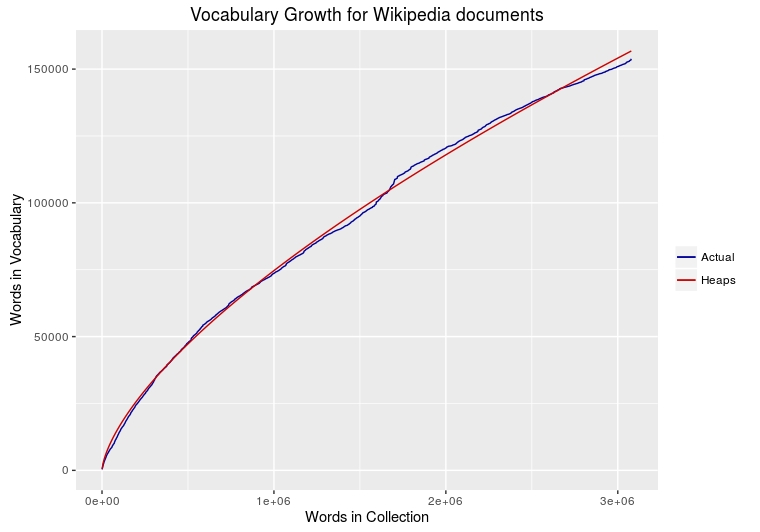
\includegraphics[scale=0.7]{4_2_ascending}}
	\centering
	\caption{Vocabulary growth for the Wikipedia Collection (Wiki small)}
	\label{fig:4_2_ascending}
\end{figure}

To find out whether or not the order of document processing affect the vocabulary growth, I modify the code so that the documents are being processed in reversed order. Figure \ref{fig:4_2_reverse} shows the plot for vocabulary growth for the Wikipedia collection in reversed order. 
\begin{figure}[H]
	\fbox{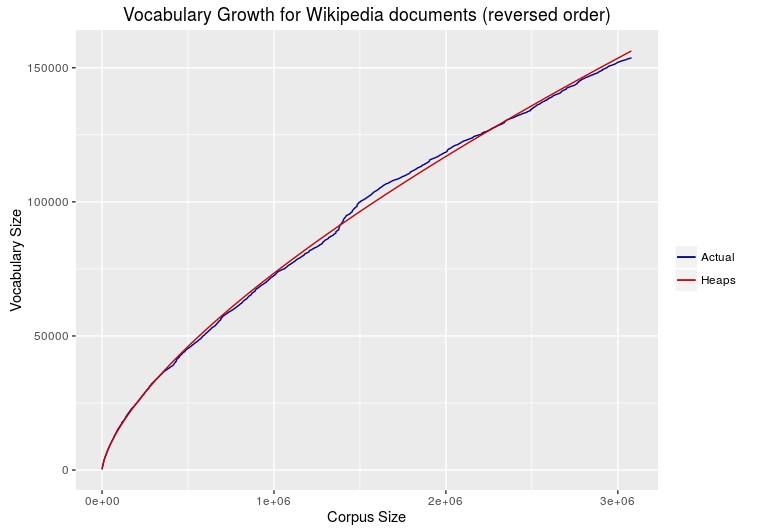
\includegraphics[scale=0.7]{4_2_reverse}}
	\centering
	\caption{Vocabulary growth for the Wikipedia Collection (Wiki small)}
	\label{fig:4_2_reverse}
\end{figure}

The complete code for calculating the vocabulary growth can be seen in listing \ref{lst:vocab-growth}

\begin{lstlisting}[language=python, caption={Source code for calculating vocabulary growth}, label={lst:vocab-growth}]
#!/usr/bin/python
import io
import os
import html2text
import unicodecsv as csv

html_files = []
# traverse the directory to list all the html files in the directory
for root, dirs, files in os.walk(os.path.abspath('./articles')):
    for file in files:
        if file.endswith('.html'):
            filepath = os.path.join(root, file)
            html_files.append(filepath)

bigrams = []
corpus = []
voc_corpus = []
# process each html file
for idx, file in enumerate(html_files):
    print('{} of {}. Processing {}'.format(idx + 1, len(html_files), file))
    print('=' * 30)

    # get text only from each file -> remove all tags
    h = html2text.HTML2Text()
    h.ignore_links = True
    text = h.handle(u' '.join([line.strip() for line in io.open(file, "r", encoding="utf-8").readlines()]))

    # get all words from text by splitting by whitespace
    tokens = []
    for word in text.split():
        if word.isalpha():
            tokens.append(word)

    # corpus is cummulative of tokens
    corpus += tokens
    # voc is unique list of corpus
    vocs = set(corpus)

    # count the size of corpus and vocabularies in the docs[file]
    voc_corpus.append([idx+1, len(corpus), len(vocs)])

print('\n\n the size of corpus {}'.format(len(corpus)))
print('\n\n the size of vocabularies {}'.format(len(vocs)))

out_file = os.path.join(os.getcwd(), '4_2-voc_corpus.csv')
with open(out_file, "wb") as f:
    writer = csv.writer(f)
    writer.writerow(["docs", "corpus_size", "vocabulary_size"])
    writer.writerows(voc_corpus)


# Process reverse list
print('\n\n Processing reverse list...')
html_files.reverse()

corpus = []
voc_corpus = []
# process each html file
for idx, file in enumerate(html_files):
    print('{} of {}. Processing {}'.format(idx + 1, len(html_files), file))
    print('=' * 30)

    # get text only from each file -> remove all tags
    h = html2text.HTML2Text()
    h.ignore_links = True
    text = h.handle(u' '.join([line.strip() for line in io.open(file, "r", encoding="utf-8").readlines()]))

    # get all words from text by splitting by whitespace
    tokens = []
    for word in text.split():
        if word.isalpha():
            tokens.append(word)

    # corpus is cummulative of tokens
    corpus += tokens
    # voc is unique list of corpus
    vocs = set(corpus)

    # count the size of corpus and vocabularies in the docs[file]
    voc_corpus.append([idx+1, len(corpus), len(vocs)])

print('\n\n the size of corpus in reverse order {}'.format(len(corpus)))
print('\n\n the size of vocabularies in reverse order {}'.format(len(vocs)))

out_file = os.path.join(os.getcwd(), '4_2-voc_corpus_reverse.csv')
with open(out_file, "wb") as f:
    writer = csv.writer(f)
    writer.writerow(["docs", "corpus_size", "vocabulary_size"])
    writer.writerows(voc_corpus)

\end{lstlisting}

Estimation of the parameters for Heap's law are done using non-linear least square (nls), which is provided in R. Table \ref{tab:heap-par} show the parameter of Heap's law both for ascending and descending order. 

\begin{table}[H]
\centering
\begin{tabular}{|l|l|l|}
\hline
\multicolumn{1}{|c|}{\textbf{No}} & \multicolumn{1}{c|}{\textbf{Parameter}} & \multicolumn{1}{c|}{\textbf{Values}} \\ \hline
1 & k ascending & 8.8941676 \\ \hline
2 & b ascending & 0.6527393 \\ \hline
3 & k descending & 7.2333319 \\ \hline
4 & b descending & 0.6663944 \\ \hline
\end{tabular}
\caption{Heap parameter for Wikipedia Collection}
\label{tab:heap-par}
\end{table}

The R code for creating the plot and calculating the parameter value can be seen in listing \ref{lst:heap-par}.

\begin{lstlisting}[language=R, caption={Code for plotting vocabulary growth and calculating the Heap's parameter}, label={lst:heap-par}]

require(ggplot2)

mydata <- read.csv("/media/erikaris/DATA/ODU/Semester 3/intro_to_info_retrieval/assignments/a2/code_report/4_2-voc_corpus.csv", head=TRUE, sep = ',')
x <- mydata$corpus_size
y <- mydata$vocabulary_size

#model
fit<-nls(y~k*(x^b), data = mydata, start = list(k=1,b=1))
summary(fit)
#get some estimation of goodness of fit
cor(y, predict(fit))

ggplot(data=mydata, aes(x=corpus_size, y=vocabulary_size))  + geom_line(aes(group = 1), color="#000099") + geom_line(data=mydata, aes(x=corpus_size, y=predict(fit)), color="#CC0000") + labs(title='Vocabulary Growth',x = 'Corpus Size', y = 'Vocabulary Size') + scale_colour_manual(name='', values=c('Important line'='grey', 'Point values'='red'), guide='legend')

#=======================================================================
# the reverse order

mydata <- read.csv("/media/erikaris/DATA/ODU/Semester 3/intro_to_info_retrieval/assignments/a2/code_report/4_2-voc_corpus_reverse.csv", head=TRUE, sep = ',')
x <- mydata$corpus_size
y <- mydata$vocabulary_size

#model
fit<-nls(y~k*(x^b), data = mydata, start = list(k=1,b=1))
summary(fit)
#get some estimation of goodness of fit
cor(y, predict(fit))

ggplot(data=mydata, aes(x=corpus_size, y=vocabulary_size))  + geom_line(aes(group = 1), color="#000099") + geom_line(data=mydata, aes(x=corpus_size, y=predict(fit)), color="#CC0000") + labs(title='Vocabulary Growth',x = 'Corpus Size', y = 'Vocabulary Size') + scale_colour_manual(name='', values=c('Important line'='grey', 'Point values'='red'), guide='legend')

\end{lstlisting}

\noindent\makebox[\linewidth]{\rule{\textwidth}{0.4pt}}

\section*{Question 4.6}
\begin{spverbatim}
Process five Wikipedia documents using the Porter stemmer and the Krovetz stemmer. Compare the number of stems produced and find 10 examples of differences in the stemming that could have an impact on ranking.
\end{spverbatim}

\subsection*{Answer}
Stemming using Porter stemmer is quite easy to do since this stemmer is provided by nltk \cite{nltk-porter}. Fortunately, there is also a python library for stemming with Krovetz algorithm \cite{krovetz-python}. So, our task now is to create a script that utilizes these 2 libraries. The logic is simple: get the text content of the documents and use Porter and Krovetz for stemming. 

To do the stemming, I randomly choose 5 documents from the Wikipedia collections. These 5 documents are:
\begin{enumerate}
\item ABC\_Wasp\_3b25.html
\item ABC\_In\_Concert\_6d5f.html
\item Abdus\_Salam\_(disambiguation)\_0602.html
\item Abd-Allah\_ibn\_Amr\_f58f.html
\item Abdul\_Haq\_Vidyarthi\_582b.html
\end{enumerate}

Figure \ref{fig:4_6_stemming_comparison} shows the comparison of stemming result between Porter and Krovetz. I circle some of the words that I consider will affect the ranking. The complete stemming result for all 5 documents is uploaded on github under a file named `4\_6-result\_rev3.txt'. 

\begin{figure}[H]
	\fbox{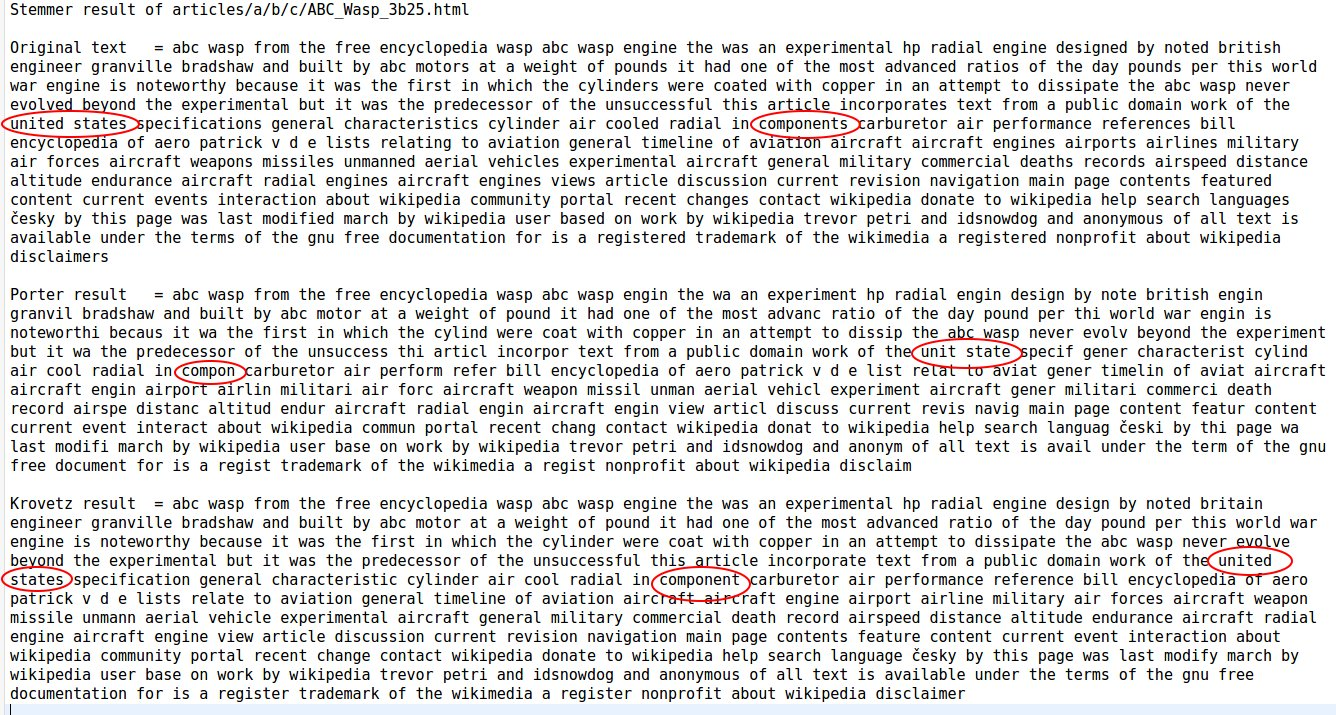
\includegraphics[scale=0.37]{4_6_stemming_comparison}}
	\centering
	\caption{Stemming comparison (Porter vs Krovetz)}
	\label{fig:4_6_stemming_comparison}
\end{figure}

Table \ref{tab:porter-krovetz} show 10 differences in the stemming between Porter and Krovetz that could have impact on ranking. From this table we can see that Porter arbitraly dissect the words. For example, Porter stem the word `united' into `unit', which have different meaning. Moreover, when this word is combined with the word next to it, they form different term. The term `united states' is clearly different with `unit state'. Therefore, we can see that it will definetely impact the ranking. 
The comparison of the number of stems produces by both Porter and Krovetz can be seen on table \ref{tab:stem}. From table \ref{tab:stem} we can see that Krovetz produced more stems compare to that of Porter. This is because Porter is more naive in `stemming' the word. So, there could be two words that are grouped together into the same stem while, in fact, they do not belong in the same stem. 

\begin{table}[H]
\centering
\begin{tabular}{|l|l|l|l|}
\hline
\rowcolor[HTML]{ECF4FF} 
\multicolumn{1}{|c|}{\cellcolor[HTML]{ECF4FF}} & \multicolumn{1}{c|}{\cellcolor[HTML]{ECF4FF}} & \multicolumn{2}{c|}{\cellcolor[HTML]{ECF4FF}\textbf{number of stems}} \\ \cline{3-4} 
\rowcolor[HTML]{ECF4FF} 
\multicolumn{1}{|c|}{\multirow{-2}{*}{\cellcolor[HTML]{ECF4FF}\textbf{No}}} & \multicolumn{1}{c|}{\multirow{-2}{*}{\cellcolor[HTML]{ECF4FF}\textbf{document}}} & Porter & Krovetz \\ \hline
1 & ABC\_Wasp\_3b25.html & 146 & 148 \\ \hline
2 & ABC\_In\_Concert\_6d5f.html & 138 & 142 \\ \hline
3 & Abdus\_Salam\_(disambiguation)\_0602.html & 91 & 93 \\ \hline
4 & Abd-Allah\_ibn\_Amr\_f58f.html & 471 & 480 \\ \hline
5 & Abdul\_Haq\_Vidyarthi\_582b.html & 165 & 170 \\ \hline
\multicolumn{2}{|c|}{\textbf{Total}} & \textbf{1011} & \textbf{1033} \\ \hline
\end{tabular}
\caption{The number of stems produced by Porter and Krovetz}
\label{tab:stem}
\end{table}

\begin{table}[H]
\centering
\begin{tabular}{|l|l|l|l|}
\hline
\rowcolor[HTML]{ECF4FF} 
\multicolumn{1}{|c|}{\cellcolor[HTML]{ECF4FF}\textbf{No}} & \multicolumn{1}{c|}{\cellcolor[HTML]{ECF4FF}\textbf{Original}} & \multicolumn{1}{c|}{\cellcolor[HTML]{ECF4FF}\textbf{Porter}} & \multicolumn{1}{c|}{\cellcolor[HTML]{ECF4FF}\textbf{Krovetz}} \\ \hline
1 & united states & unit state & united states \\ \hline
2 & available & avail & available \\ \hline
3 & engine & engin & engine \\ \hline
4 & component & compon & component \\ \hline
5 & airspeed & airspe & airspeed \\ \hline
6 & movie & movi & movie \\ \hline
7 & tradition & tradit & tradit \\ \hline
8 & eventually & eventu & eventually \\ \hline
9 & since & sinc & since \\ \hline
10 & navigation & navig & navigation \\ \hline
\end{tabular}
\caption{Examples of differences in stemming between Porter and Krovetz}
\label{tab:porter-krovetz}
\end{table}

The source code for processing the Porter and Krovetz stemmer can be seen in listing \ref{lst:porter-krovetz}.

\begin{lstlisting}[language=python, caption={Source code for stemming document using Porter Stemmer and Krovetz Stemmer}, label={lst:porter-krovetz}]

#!/usr/bin/python
import io
import sys

import html2text as html2text
import krovetzstemmer
from nltk import PorterStemmer

# Instantiate porter stemmer
porter = PorterStemmer()
krovetz = krovetzstemmer.Stemmer()

if len(sys.argv) < 6:
    print('Usage :')
    print('python 4_6.py <file_1> ... <file_5>')

# Assuming all arguments are file
files = []
for arg in range(1, len(sys.argv)):
    files.append(sys.argv[arg])

# Get contents of each file
results = {}
for idx, file in enumerate(files):
    print('{} of {}. Processing {}'.format(idx + 1, len(files), file))
    print('=' * 30)

    # get text content
    h = html2text.HTML2Text()
    h.ignore_links = True
    text = h.handle(u' '.join([line.strip() for line in io.open(file, "r", encoding="utf-8").readlines()]))

    # remove whitespace
    words = []
    for word in text.split():
        if word.isalpha():
            words.append(word.lower())
    text = u' '.join(words)

    porter_result = []
    krovetz_result = []
    for c in words:
        porter_result.append(porter.stem(c))
        krovetz_result.append(krovetz.stem(c))

    results[file] = {}
    results[file]['original'] = text
    results[file]['porter'] = u' '.join(porter_result)
    results[file]['krovetz'] = u' '.join(krovetz_result)

# print results
txt_results = []
for file in results:
    txt_results.append(u'Stemmer result of {}'.format(file))
    txt_results.append(u'{}'.format('=' * 60))
    txt_results.append(u'Original text \t= {}\n'.format(results[file]['original']))
    txt_results.append(u'Porter result \t= {}\n'.format(results[file]['porter']))
    txt_results.append(u'Krovetz result \t= {}\n'.format(results[file]['krovetz']))

    num_stems_porter = len(set(results[file]['porter'].split()))
    txt_results.append(u'Number of stems produced by Porter \t= {}\n'.format(num_stems_porter))

    num_stems_krovetz = len(set(results[file]['krovetz'].split()))
    txt_results.append(u'Number of stems produced by Krovetz \t= {}\n'.format(num_stems_krovetz))
    txt_results.append(u'\n')

    print(u'\n'.join(txt_results))

    # also write to file
    f = io.open('4_6-result.txt', "w", encoding="utf-8")
    for txt_result in txt_results:
        f.write(txt_result + '\n')

\end{lstlisting}

\noindent\makebox[\linewidth]{\rule{\textwidth}{0.4pt}}

\section*{Question 4.8}
\begin{spverbatim}
Find the 10 Wikipedia documents with the most inlinks. Show the collection of anchor text for those pages.
\end{spverbatim}

\subsection*{Answer}
Here is the algorithm to find the document with the most inlinks:
\begin{enumerate}
\item Use Beautiful Soup \cite{bs4} to extract all links from the Wikipedia documents.
\item Store the links in a key-value format, where key = document and value = link. 
\item Group and count the links by the destination (the one that is written in `href'). This will be the number of inlinks for each destination. 
\item Sort the data by the number of inlinks in a descending order.  
\end{enumerate}

Table \ref{tab:inlinks} shows 10 Wikipedia documents with the most inlinks and their anchor text. 

\begin{table}[H]
\centering
\begin{tabular}{|l|l|l|l|}
\hline
\multicolumn{1}{|c|}{\textbf{No}} & \multicolumn{1}{c|}{\textbf{Link}} & \multicolumn{1}{c|}{\textbf{Inlinks}} & \multicolumn{1}{c|}{\textbf{Anchor Text}} \\ \hline
1 & Brazil.html & 83 & Brazil, BRA, Brazilian \\ \hline
2 & August\_26.html & 25 & 08-26, 26, August 26, 26 August \\ \hline
3 & Manga.html & 14 & manga, Manga \\ \hline
4 & Magazine.html & 13 & magazine, magazines, Magazine \\ \hline
5 & Mollusca.html & 12 & Mollusca \\ \hline
6 & Victoria\_of\_the\_United\_Kingdom\_5e8e.html & 8 & \begin{tabular}[c]{@{}l@{}}Queen Victoria, Queen,\\ Victoria of the United Kingdom, Victoria\end{tabular} \\ \hline
7 & Screenwriter.html & 7 & Writer(s), screenwriter, Screenwriter \\ \hline
8 & Kidney.html & 6 & kidneys, Renal, kidney \\ \hline
9 & Tottenham\_Hotspur\_F.C.\_6bd2.html & 5 & Tottenham Hotspur, Tottenham \\ \hline
10 & Tuscany.html & 4 & Tuscany \\ \hline
\end{tabular}
\caption{Wikipedia documents with the most inlinks}
\label{tab:inlinks}
\end{table}

The complete source code for processing the inlinks can be seen in listing \ref{lst:inlinks}.

\begin{lstlisting}[language=python, caption={Source code for finding 10 Wikipedia documents with the most inlinks}, label={lst:inlinks}]

#!/usr/bin/python
import os
from pprint import pprint

import unicodecsv as csv
from bs4 import BeautifulSoup
from tabulate import tabulate

html_files = []
# traverse the directory to list all the html files in the directory
for root, dirs, files in os.walk(os.path.abspath('./articles')):
    for file in files:
        if file.endswith('.html'):
            filepath = os.path.join(root, file)
            html_files.append(filepath)

all_links = {}
all_anchor_text = {}
# process each html file
for idx, file in enumerate(html_files):
    # just for debugging
    print('{} of {}. Processing {}'.format(idx+1, len(html_files), file))
    print('=' * 30)

    # find all anchors
    soup = BeautifulSoup(open(file), 'html.parser')
    anchors = soup.find_all('a', href=True)
    print('Found {} anchors'.format(len(anchors)))

    for a in anchors:
        link = a['href']
        # anchor text
        text = a.string or ''

        # In this case, link is relative path points to other html file
        # just process non http link
        if not link.startswith('http'):
            try:
                # convert to absolute path
                link = os.path.join(os.path.dirname(file), link)
                link = os.path.abspath(link)
            except:
                pass

        # all_link : key is source, value is list of destination
        all_links.setdefault(file, [])
        # all_anchor_text : key is source, value is list of anchor text
        all_anchor_text.setdefault(file, [])

        # append only if:
        # - file != link
        # - all_links do not contain link
        # - link is file --> ignore http
        if file != link and link not in all_links[file] and os.path.isfile(link):
            all_links[file].append(link)
            all_anchor_text[file].append(text)

link_freq = {}
link_text = {}
for src in all_links:
    # all destinations in each src
    dests = all_links[src]
    # all anchor text in each src
    texts = all_anchor_text[src]

    for idx, dest in enumerate(dests):
        link_freq.setdefault(dest, 0)
        link_freq[dest] += 1

        link_text.setdefault(dest, [])
        link_text[dest].append(texts[idx])

# convert dict to 2d list
link_freq_table = []
for link in link_freq:
    link_freq_table.append([link, link_freq[link]])

# sort list by freq (2nd column)
link_freq_table = sorted(link_freq_table, key=lambda x:x[1], reverse=True)

# append anchor texts in 3rd column
tmp_link_freq_table = []
for row in link_freq_table:
    # append anchor texts in 3rd column
    row += [u', '.join(set(link_text[row[0]]))]
    # convert full-path link to filename only
    row[0] = os.path.basename(row[0])
    tmp_link_freq_table.append(row)
link_freq_table = tmp_link_freq_table

# process only top 10 results
link_freq_table = link_freq_table[:10]

# write the output to csv file
out_file = os.path.join(os.getcwd(), '4_8-link_freq.csv')
with open(out_file, "wb") as f:
    writer = csv.writer(f)
    writer.writerow(["link", "frequency", "texts"])
    writer.writerows(link_freq_table)

# print the resulting table
print tabulate(link_freq_table, headers=["link", "frequency", "texts"])
\end{lstlisting}

\noindent\makebox[\linewidth]{\rule{\textwidth}{0.4pt}}


\section*{Question 5.8}
\begin{spverbatim}
Write a program that can build a simple inverted index of a set of text documents. Each inverted list will contain the file names of the documents that contain that word.
Suppose the file A contains the text “the quick brown fox”, and file B contains
“the slow blue fox”. The output of your program would be:

% ./your-program A B

blue B
brown A
fox A B
quick A
slow B
the A B
\end{spverbatim}

\subsection*{Answer}
To create an inverted index, we need to `swap' the role of words vs documents. There are many nice examples that we can find on the internet about how to create inverted index. One that I find easier to understand is the one provided by RosettaCode.org \cite{rosetta}. The algorithm is quite simple:
\begin{enumerate}
\item List all words in each document. We will get a key-value pair, where document is the key and words are the value. 
\item `Swap' the role of words and documents. Now, word is the key and document is the value. 
\item Write the output to a csv file. 
\end{enumerate}

The source code for the inverted index can be seen in listing \ref{lst:inverted-index}. This code run using terminal input (figure \ref{fig:5_8_terminal_input}). 

\begin{figure}[H]
	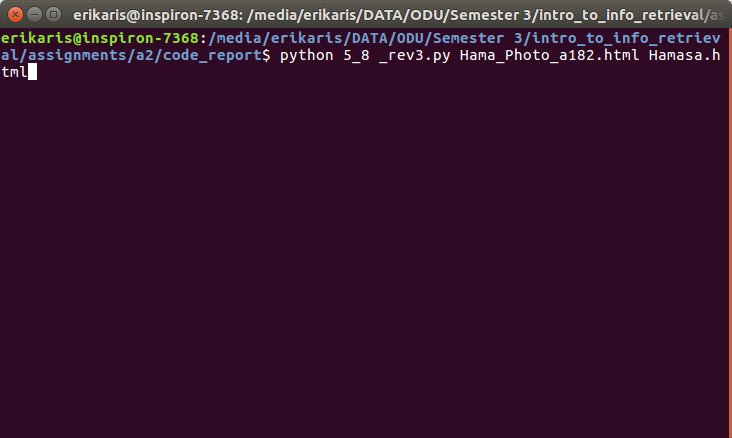
\includegraphics[scale=0.6]{5_8_terminal_input}
	\caption{Terminal input for running the inverted index}
	\label{fig:5_8_terminal_input}
\end{figure}

\begin{lstlisting}[language=python, caption={Source code for simple inverted index}, label={lst:inverted-index}]

#!/usr/bin/python
import unicodecsv as csv
import io
import os
import sys

import html2text
from tabulate import tabulate

# Assuming all arguments are file
files = []
for arg in range(1, len(sys.argv)):
    files.append(sys.argv[arg])

file_words_index = {}
all_words = set()

# Read all files
for file in files:
    # get text content
    h = html2text.HTML2Text()
    h.ignore_links = True
    text = h.handle(u' '.join([line.strip() for line in io.open(file, "r", encoding="utf-8").readlines()]))

    words = [word.lower() for word in text.split() if word.isalpha()]
    all_words |= set(words)
    file_words_index[file.split(os.pathsep)[-1]] = words

# Invert words and files
word_files_index = {}
for word in all_words:
    files = []
    for file, words in file_words_index.items():
        if word in words:
            files.append(file)
    word_files_index[word] = sorted(set(files))

# Convert to 2d array
table = []
for word in word_files_index:
    table.append([word, u', '.join(word_files_index[word])])

print tabulate(table, headers=["word", "files"])

# write the output to csv file
out_file = os.path.join(os.getcwd(), '5_8-inverted_index.csv')
with open(out_file, "wb") as f:
    writer = csv.writer(f)
    writer.writerow(["word", "files"])
    writer.writerows(table)
\end{lstlisting}

Table \ref{tab:inverted-index} shows 20 first rows of the inverted index created from Wikipedia document `Hama\_Photo\_a182.html' and `Hamasa.html'. These 2 Wikipedia documents are chosen randomly. The complete list of the inverted index is uploaded on github under file named `5\_8-inverted\_index\_rev1.csv'.

\begin{table}[H]
\centering
\begin{tabular}{|l|l|l|}
\hline
\rowcolor[HTML]{ECF4FF} 
\multicolumn{1}{|c|}{\cellcolor[HTML]{ECF4FF}\textbf{No}} & \multicolumn{1}{c|}{\cellcolor[HTML]{ECF4FF}\textbf{word}} & \multicolumn{1}{c|}{\cellcolor[HTML]{ECF4FF}\textbf{documents}} \\ \hline
1 & all & \begin{tabular}[c]{@{}l@{}}articles/h/a/m/Hama\_Photo\_a182.html, \\ articles/h/a/m/Hamasa.html\end{tabular} \\ \hline
2 & help & \begin{tabular}[c]{@{}l@{}}articles/h/a/m/Hama\_Photo\_a182.html, \\ articles/h/a/m/Hamasa.html\end{tabular} \\ \hline
3 & german & articles/h/a/m/Hama\_Photo\_a182.html \\ \hline
4 & photo & articles/h/a/m/Hama\_Photo\_a182.html \\ \hline
5 & supported & articles/h/a/m/Hamasa.html \\ \hline
6 & founded & articles/h/a/m/Hama\_Photo\_a182.html \\ \hline
7 & including & articles/h/a/m/Hama\_Photo\_a182.html \\ \hline
8 & filters & articles/h/a/m/Hama\_Photo\_a182.html \\ \hline
9 & world & articles/h/a/m/Hama\_Photo\_a182.html \\ \hline
10 & pvac & articles/h/a/m/Hama\_Photo\_a182.html \\ \hline
11 & bombing & articles/h/a/m/Hama\_Photo\_a182.html \\ \hline
12 & current & \begin{tabular}[c]{@{}l@{}}articles/h/a/m/Hama\_Photo\_a182.html, \\ articles/h/a/m/Hamasa.html\end{tabular} \\ \hline
13 & based & \begin{tabular}[c]{@{}l@{}}articles/h/a/m/Hama\_Photo\_a182.html, \\ articles/h/a/m/Hamasa.html\end{tabular} \\ \hline
14 & equipment & articles/h/a/m/Hama\_Photo\_a182.html \\ \hline
15 & flash & articles/h/a/m/Hama\_Photo\_a182.html \\ \hline
16 & hanke & articles/h/a/m/Hama\_Photo\_a182.html \\ \hline
17 & languages & articles/h/a/m/Hama\_Photo\_a182.html \\ \hline
18 & to & \begin{tabular}[c]{@{}l@{}}articles/h/a/m/Hama\_Photo\_a182.html, \\ articles/h/a/m/Hamasa.html\end{tabular} \\ \hline
19 & under & \begin{tabular}[c]{@{}l@{}}articles/h/a/m/Hama\_Photo\_a182.html, \\ articles/h/a/m/Hamasa.html\end{tabular} \\ \hline
20 & extensive & articles/h/a/m/Hama\_Photo\_a182.html \\ \hline
\end{tabular}
\caption{20 first rows of the inverted index created from 2 Wikipedia documents}
\label{tab:inverted-index}
\end{table}

\medskip

\bibliographystyle{unsrt}%Used BibTeX style is unsrt
\bibliography{biblio}

\end{document}
